\subsection{Instrumentation}

	PXRD diffractometers can be broadly classified into two types:%
%	
	\begin{enumerate}%
%	
	    \item the reflection geometry, and
	    
	    \item the transmission or Debye-Scherrer geometry.
	    
	\end{enumerate}
	
	\begin{figure}
		\centering
		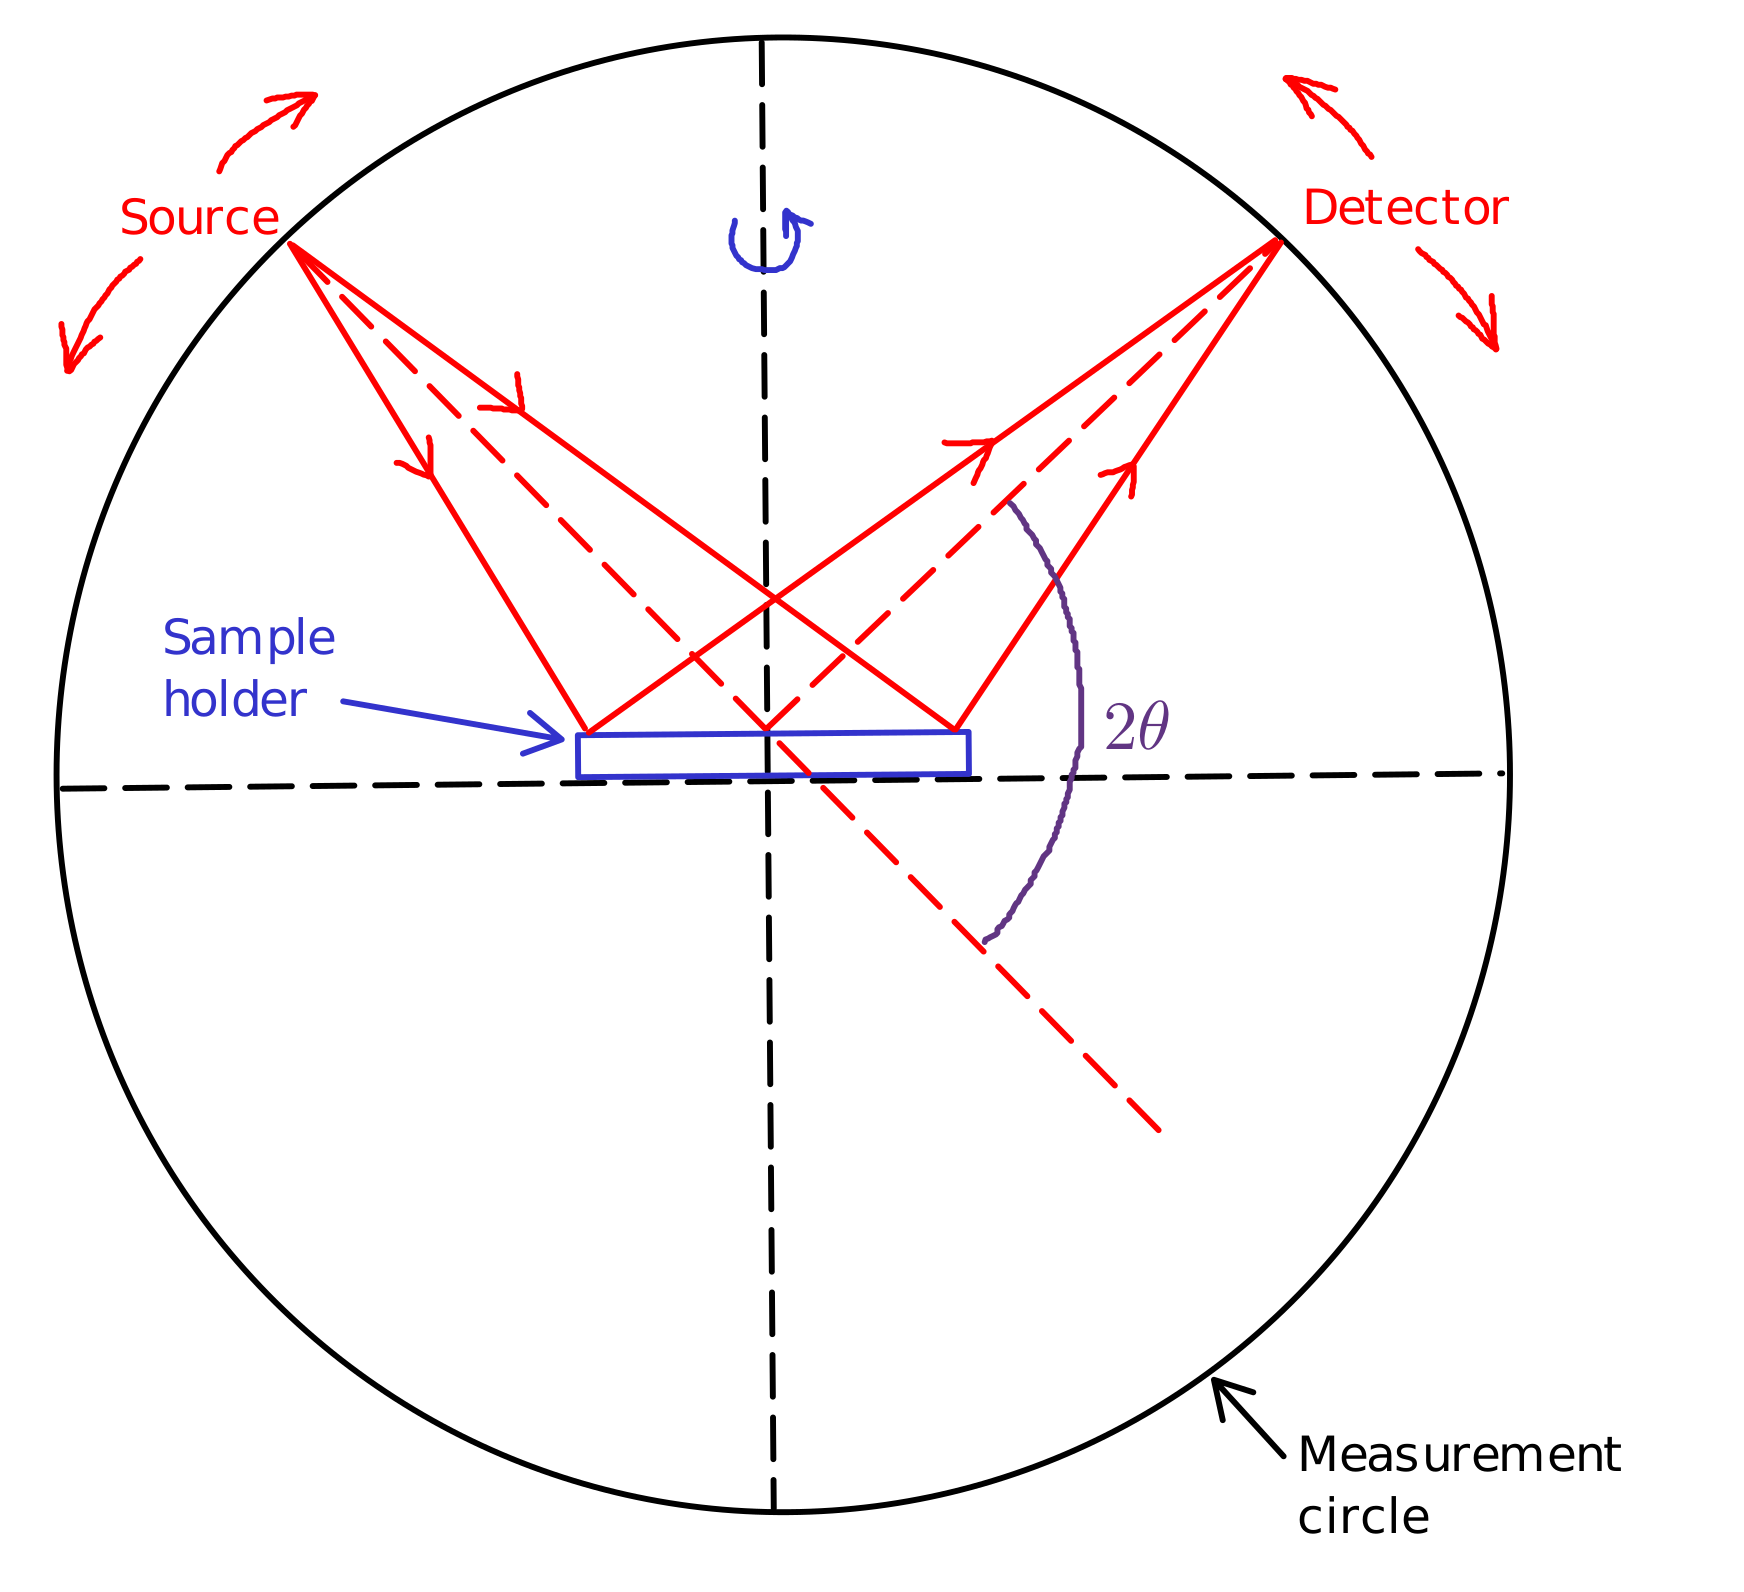
\includegraphics[scale=0.15]{bragg_bretano_diff.png}
		\caption{\label{fig:bragg_bretano_diff}Schematic of a reflection-type Bragg-Bretano diffractometer.}
	\end{figure}
	
	Figure~\ref{fig:bragg_bretano_diff} shows the schematic of a reflection geometry-based powder X-ray diffractometer. The sample holder is rotated in the presence of the beam to remove any special orientation effect. In PXRD, we do not use a circularly focussed beam, instead, we use a line beam, with the line falling on the sample. There are two geometries based on how the line beam is created:%
%	
	\begin{enumerate}%
%	
	    \item The Bragg-Brentano (BB) geometry, which uses a diverging beam.
	    
	    \item The parallel beam (PB) geometry, which uses a parallel beam of X-rays.
	    
	\end{enumerate}
	
	\begin{figure}
		\centering
		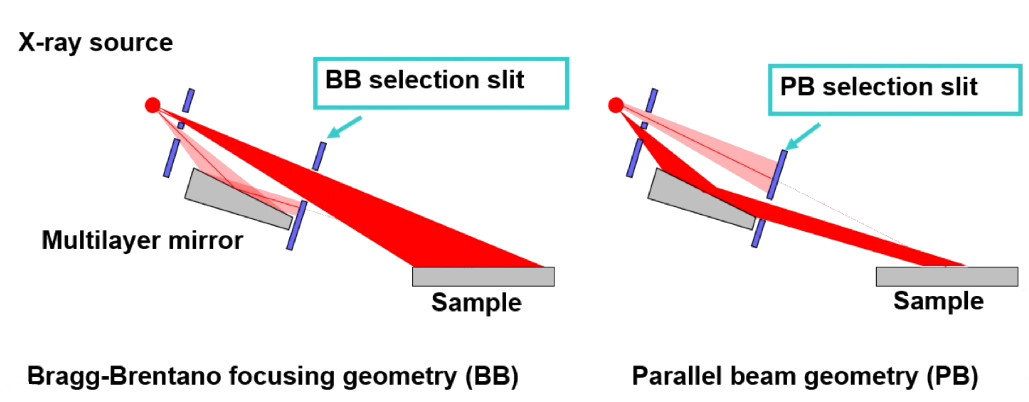
\includegraphics[width=\textwidth]{cross_beam_optics.png}
		\caption{\label{fig:cross_beam_optics}Bragg-Bretano (BB) and parallel beam (PB) geometry. Cross Beam Optics is a patented technology by Rigaku Oxford Diffractometers. The BB and PB geometries are simultaneously mounted, aligned and selectable by the means of a removable slit. Design taken from \cite{Chowdhury2022}.}
	\end{figure}
	
	This Cross Beam Optics is shown in figure~\ref{fig:cross_beam_optics}. The PB geometry is particularly useful when we have a small amount of sample, and we want to focus the X-rays on the sample only and want to avoid the diffraction of the sample holder plate.
	
	 The Bragg-Brentano diffractometers can further be of two types, as listed in table~\ref{tab:bragg_bretano}
	 . In the $\theta : 2\theta$ type, the X-ray source is fixed, while the specimen holder and the detector are both rotated. The detector moves by an angle $2\theta$ when the sample holder moves by $\theta.$ In the $\theta : \theta$ geometry, the specimen is kept fixed, while the tube and the detector are moved together in opposite directions (i.e. both towards or away from each other).
	 
	\begin{table}
	
		\centering
		
		\caption{\label{tab:bragg_bretano}Types of Bragg-Bretano diffractometers.}
		\begin{tabular}{|c|c|c|c|}
		
			\hline
			
			Type & X-ray tube & Specimen holder & Detector \\
			
			\hhline{|=|=|=|=|}
			
			$\theta : 2\theta$ & Fixed & Varies as $\theta$ & Varies as $2\theta$ \\
			
			\hline
			
			$\theta : \theta$ & Varies as $\theta$ & Fixed & Varies as $\theta$ \\
			
			\hline
		
		\end{tabular}
	\end{table}
	
	The Debye-Scherrer diffractometers are transmission-type diffractometers in which the X-rays pass through the sample and are recorded by the detector on the other side. These are used when the sample does not absorb X-rays, and are particularly useful if the sample is loaded in a capillary tube.
	
\subsection{Data collection}

	Collecting high quality data is the primary requirement in PXRD experiments. We need to keep a few points in mind in these experiments:%
%		
		\begin{enumerate}%
%		
		    \item \bfnt{Sample quality}: The sample must be free-flowing powder, must not be moisture sensitive, and must ideally contain no moisture. Presence of moisture will change the background in the recorded data.
		    
		    \item \bfnt{Range of $2\theta$}: This will not be known \textit{a priori}. Initially, we collect data upto an approximate range, and based on the peaks, we decrease the step size and focus on a certain range. For organic and organometallic samples, we generally record in the range $3-50~\si{\degree}$ in $2\theta,$ while for inorganic samples, we often go up to around $\SI{100}{\degree}.$
		    
		    \item \bfnt{Scan speed}: Scan speed can vary from as high as $\SI{20}{\degree}$ in $\si{2\theta \per min}$ to as low as $\SI{0.2}{\degree}$ in $\si{2\theta \per min}.$
		    
		    \item \bfnt{Step size}: Step sizes can vary between $\SI{0.1}{\degree}$ in $2\theta$ to as low as $\SI{0.001}{\degree}$ in $2\theta.$ We must ensure that the scan speed and step size combination is such that sufficient time is allowed to resolve each and every peak.
		    
		    \item \bfnt{Sample rotation}: Due to spreading process of the powdered sample on the sample plate, it may happen that one side of the sample is generating unusually higher peaks compared to the other. This is called the preferred orientation effect. It is necessary to rotate the sample to get rid of this. Normally, a rotation speed of $100-120~\si{rpm}$ speed is used.
		    
		    \item \bfnt{Monochromator}: Generally, PXRD diffractometers are not equipped with a \\monochromator, but we can use one. However, the intensity of the peaks reduces drastically in that case.
		    
		\end{enumerate}
		
	Overlapping of peaks is one of the very common issues in PXRD, and it is very difficult to separate such overlapped peaks. Indexing is a much harder work, and is often done using the Inorganic Crystal Structure Database (ICSD) and the Organic Powder Structural Database, maintained by the International Centre for Diffraction Data (ICDD). Using this database, impurities can also be identified in many cases. We shall not go into the details of indexing using software for PXRD.
	